\documentclass[]{article}
\usepackage{lmodern}
\usepackage{amssymb,amsmath}
\usepackage{ifxetex,ifluatex}
\usepackage{fixltx2e} % provides \textsubscript
\ifnum 0\ifxetex 1\fi\ifluatex 1\fi=0 % if pdftex
  \usepackage[T1]{fontenc}
  \usepackage[utf8]{inputenc}
\else % if luatex or xelatex
  \ifxetex
    \usepackage{mathspec}
  \else
    \usepackage{fontspec}
  \fi
  \defaultfontfeatures{Ligatures=TeX,Scale=MatchLowercase}
\fi
% use upquote if available, for straight quotes in verbatim environments
\IfFileExists{upquote.sty}{\usepackage{upquote}}{}
% use microtype if available
\IfFileExists{microtype.sty}{%
\usepackage{microtype}
\UseMicrotypeSet[protrusion]{basicmath} % disable protrusion for tt fonts
}{}
\usepackage[margin=1in]{geometry}
\usepackage{hyperref}
\hypersetup{unicode=true,
            pdftitle={Course 6 Project - Statistical Inference - PART 1},
            pdfauthor={majusus},
            pdfborder={0 0 0},
            breaklinks=true}
\urlstyle{same}  % don't use monospace font for urls
\usepackage{color}
\usepackage{fancyvrb}
\newcommand{\VerbBar}{|}
\newcommand{\VERB}{\Verb[commandchars=\\\{\}]}
\DefineVerbatimEnvironment{Highlighting}{Verbatim}{commandchars=\\\{\}}
% Add ',fontsize=\small' for more characters per line
\usepackage{framed}
\definecolor{shadecolor}{RGB}{248,248,248}
\newenvironment{Shaded}{\begin{snugshade}}{\end{snugshade}}
\newcommand{\KeywordTok}[1]{\textcolor[rgb]{0.13,0.29,0.53}{\textbf{#1}}}
\newcommand{\DataTypeTok}[1]{\textcolor[rgb]{0.13,0.29,0.53}{#1}}
\newcommand{\DecValTok}[1]{\textcolor[rgb]{0.00,0.00,0.81}{#1}}
\newcommand{\BaseNTok}[1]{\textcolor[rgb]{0.00,0.00,0.81}{#1}}
\newcommand{\FloatTok}[1]{\textcolor[rgb]{0.00,0.00,0.81}{#1}}
\newcommand{\ConstantTok}[1]{\textcolor[rgb]{0.00,0.00,0.00}{#1}}
\newcommand{\CharTok}[1]{\textcolor[rgb]{0.31,0.60,0.02}{#1}}
\newcommand{\SpecialCharTok}[1]{\textcolor[rgb]{0.00,0.00,0.00}{#1}}
\newcommand{\StringTok}[1]{\textcolor[rgb]{0.31,0.60,0.02}{#1}}
\newcommand{\VerbatimStringTok}[1]{\textcolor[rgb]{0.31,0.60,0.02}{#1}}
\newcommand{\SpecialStringTok}[1]{\textcolor[rgb]{0.31,0.60,0.02}{#1}}
\newcommand{\ImportTok}[1]{#1}
\newcommand{\CommentTok}[1]{\textcolor[rgb]{0.56,0.35,0.01}{\textit{#1}}}
\newcommand{\DocumentationTok}[1]{\textcolor[rgb]{0.56,0.35,0.01}{\textbf{\textit{#1}}}}
\newcommand{\AnnotationTok}[1]{\textcolor[rgb]{0.56,0.35,0.01}{\textbf{\textit{#1}}}}
\newcommand{\CommentVarTok}[1]{\textcolor[rgb]{0.56,0.35,0.01}{\textbf{\textit{#1}}}}
\newcommand{\OtherTok}[1]{\textcolor[rgb]{0.56,0.35,0.01}{#1}}
\newcommand{\FunctionTok}[1]{\textcolor[rgb]{0.00,0.00,0.00}{#1}}
\newcommand{\VariableTok}[1]{\textcolor[rgb]{0.00,0.00,0.00}{#1}}
\newcommand{\ControlFlowTok}[1]{\textcolor[rgb]{0.13,0.29,0.53}{\textbf{#1}}}
\newcommand{\OperatorTok}[1]{\textcolor[rgb]{0.81,0.36,0.00}{\textbf{#1}}}
\newcommand{\BuiltInTok}[1]{#1}
\newcommand{\ExtensionTok}[1]{#1}
\newcommand{\PreprocessorTok}[1]{\textcolor[rgb]{0.56,0.35,0.01}{\textit{#1}}}
\newcommand{\AttributeTok}[1]{\textcolor[rgb]{0.77,0.63,0.00}{#1}}
\newcommand{\RegionMarkerTok}[1]{#1}
\newcommand{\InformationTok}[1]{\textcolor[rgb]{0.56,0.35,0.01}{\textbf{\textit{#1}}}}
\newcommand{\WarningTok}[1]{\textcolor[rgb]{0.56,0.35,0.01}{\textbf{\textit{#1}}}}
\newcommand{\AlertTok}[1]{\textcolor[rgb]{0.94,0.16,0.16}{#1}}
\newcommand{\ErrorTok}[1]{\textcolor[rgb]{0.64,0.00,0.00}{\textbf{#1}}}
\newcommand{\NormalTok}[1]{#1}
\usepackage{graphicx,grffile}
\makeatletter
\def\maxwidth{\ifdim\Gin@nat@width>\linewidth\linewidth\else\Gin@nat@width\fi}
\def\maxheight{\ifdim\Gin@nat@height>\textheight\textheight\else\Gin@nat@height\fi}
\makeatother
% Scale images if necessary, so that they will not overflow the page
% margins by default, and it is still possible to overwrite the defaults
% using explicit options in \includegraphics[width, height, ...]{}
\setkeys{Gin}{width=\maxwidth,height=\maxheight,keepaspectratio}
\IfFileExists{parskip.sty}{%
\usepackage{parskip}
}{% else
\setlength{\parindent}{0pt}
\setlength{\parskip}{6pt plus 2pt minus 1pt}
}
\setlength{\emergencystretch}{3em}  % prevent overfull lines
\providecommand{\tightlist}{%
  \setlength{\itemsep}{0pt}\setlength{\parskip}{0pt}}
\setcounter{secnumdepth}{0}
% Redefines (sub)paragraphs to behave more like sections
\ifx\paragraph\undefined\else
\let\oldparagraph\paragraph
\renewcommand{\paragraph}[1]{\oldparagraph{#1}\mbox{}}
\fi
\ifx\subparagraph\undefined\else
\let\oldsubparagraph\subparagraph
\renewcommand{\subparagraph}[1]{\oldsubparagraph{#1}\mbox{}}
\fi

%%% Use protect on footnotes to avoid problems with footnotes in titles
\let\rmarkdownfootnote\footnote%
\def\footnote{\protect\rmarkdownfootnote}

%%% Change title format to be more compact
\usepackage{titling}

% Create subtitle command for use in maketitle
\providecommand{\subtitle}[1]{
  \posttitle{
    \begin{center}\large#1\end{center}
    }
}

\setlength{\droptitle}{-2em}

  \title{Course 6 Project - Statistical Inference - PART 1}
    \pretitle{\vspace{\droptitle}\centering\huge}
  \posttitle{\par}
    \author{majusus}
    \preauthor{\centering\large\emph}
  \postauthor{\par}
      \predate{\centering\large\emph}
  \postdate{\par}
    \date{April 7, 2019}


\begin{document}
\maketitle

\section{Git repository}\label{git-repository}

\section{Synopsis}\label{synopsis}

This is a project for the Coursera Statistical Inference Class. The
project consists of two parts:

\begin{verbatim}
1.Simulation Exercise to explore inference
2.Basic inferential analysis using the ToothGrowth data in the R datasets package 
\end{verbatim}

\section{Part 1 - Simulation
Exercise}\label{part-1---simulation-exercise}

\subsection{Overview}\label{overview}

Investigate the exponential distribution in R and compare it with the
Central Limit Theorem. The exponential distribution can be simulated in
R with rexp(n, lambda) where lambda is the rate parameter. The mean of
exponential distribution is 1/lambda and the standard deviation is also
1/lambda. Set lambda = 0.2 for all of the simulations. You will
investigate the distribution of averages of 40 exponentials. Note that
you will need to do a thousand simulations.

\subsection{Instructions}\label{instructions}

\begin{enumerate}
\def\labelenumi{\arabic{enumi}.}
\tightlist
\item
  Show the sample mean and compare it to the theoretical mean of the
  distribution.
\item
  Show how variable the sample is (via variance) and compare it to the
  theoretical variance of the distribution.
\item
  Show that the distribution is approximately normal.
\end{enumerate}

\subsection{Prepare Environment}\label{prepare-environment}

Load Libraries and set Global Options.

\begin{Shaded}
\begin{Highlighting}[]
\CommentTok{#To suppress loading messages set *message = FALSE*. }
\CommentTok{#Set global options *echo = TRUE* so others will be able to read the code and set *results = hold* to hold & push output to end of chunk.}
\KeywordTok{library}\NormalTok{(knitr)}
\NormalTok{opts_chunk}\OperatorTok{$}\KeywordTok{set}\NormalTok{(}\DataTypeTok{echo =} \OtherTok{TRUE}\NormalTok{, }\DataTypeTok{results =} \StringTok{'hold'}\NormalTok{)}
\KeywordTok{library}\NormalTok{(data.table)}
\KeywordTok{library}\NormalTok{(ggplot2)}
\end{Highlighting}
\end{Shaded}

Set variables as defined in the problem.

\begin{Shaded}
\begin{Highlighting}[]
\NormalTok{n <-}\StringTok{ }\DecValTok{40} \CommentTok{# number of exponentials (sample size)}
\NormalTok{lambda <-}\StringTok{ }\FloatTok{0.2} \CommentTok{# lambda for rexp (limiting factor) (rate)}
\NormalTok{nosim <-}\StringTok{ }\DecValTok{1000} \CommentTok{# number of simulations}
\NormalTok{quantile <-}\StringTok{ }\FloatTok{1.96} \CommentTok{# 95th % quantile to be used in Confidence Interval}
\KeywordTok{set.seed}\NormalTok{(}\DecValTok{234}\NormalTok{) }\CommentTok{# set the seed value for reproducibility}
\end{Highlighting}
\end{Shaded}

Create a matrix with 1000 simulations each with 40 samples drawn from
the exponential distribution.

\begin{Shaded}
\begin{Highlighting}[]
\CommentTok{# Use rexp() and matrix() to generate 40 samples creating a matrix with 1000 rows and 40 columns.}
\NormalTok{simData <-}\StringTok{ }\KeywordTok{matrix}\NormalTok{(}\KeywordTok{rexp}\NormalTok{(n }\OperatorTok{*}\StringTok{ }\NormalTok{nosim, }\DataTypeTok{rate =}\NormalTok{ lambda), nosim)}
\end{Highlighting}
\end{Shaded}

Calculate the averages across the 40 values for each of the 1000
simulations.

\begin{Shaded}
\begin{Highlighting}[]
\NormalTok{simMeans <-}\StringTok{ }\KeywordTok{rowMeans}\NormalTok{(simData) }\CommentTok{# Matrix Mean}
\end{Highlighting}
\end{Shaded}

\subsection{Mean Comparison}\label{mean-comparison}

Show the sample mean and compare it to the theoretical mean of the
distribution.

\subsubsection{Sample Mean}\label{sample-mean}

Calculate the actual mean of sample data; the average sample mean of
1000 simulations of 40 randomly sampled exponential distributions.

\begin{Shaded}
\begin{Highlighting}[]
\NormalTok{sampleMean <-}\StringTok{ }\KeywordTok{mean}\NormalTok{(simMeans) }\CommentTok{# Mean of sample means}
\NormalTok{sampleMean}
\end{Highlighting}
\end{Shaded}

\begin{verbatim}
## [1] 5.001573
\end{verbatim}

\subsubsection{Theoretical Mean}\label{theoretical-mean}

Calculate the theoretical mean; the expected mean of the exponential
distribution of rate = 1/lambda.

\begin{Shaded}
\begin{Highlighting}[]
\NormalTok{theoMean <-}\StringTok{ }\DecValTok{1} \OperatorTok{/}\StringTok{ }\NormalTok{lambda }\CommentTok{# Theoretical Mean}
\NormalTok{theoMean}
\end{Highlighting}
\end{Shaded}

\begin{verbatim}
## [1] 5
\end{verbatim}

The distribution of the mean of the sample means is centered at
\textbf{5.001573} and the theoretical mean is centered at \textbf{5}.
The mean of the sample means and the theoretical mean (expected mean)
are very close.

\subsection{Variance Comparison}\label{variance-comparison}

Show how variable the sample is and compare it to the theoretical
variance of the distribution.

\subsubsection{Sample Variance}\label{sample-variance}

Calculate the Actual Variance.

\begin{Shaded}
\begin{Highlighting}[]
\NormalTok{sampleVar <-}\StringTok{ }\KeywordTok{var}\NormalTok{(simMeans)}
\NormalTok{sampleVar}
\end{Highlighting}
\end{Shaded}

\begin{verbatim}
## [1] 0.6631504
\end{verbatim}

\subsubsection{Theoretical Variance}\label{theoretical-variance}

Calculate the theoretical variance (expected variance).

\begin{Shaded}
\begin{Highlighting}[]
\NormalTok{theoVar  <-}\StringTok{ }\NormalTok{(}\DecValTok{1} \OperatorTok{/}\StringTok{ }\NormalTok{lambda)}\OperatorTok{^}\DecValTok{2} \OperatorTok{/}\StringTok{ }\NormalTok{(n) }
\NormalTok{theoVar}
\end{Highlighting}
\end{Shaded}

\begin{verbatim}
## [1] 0.625
\end{verbatim}

The variance of the sample means is \textbf{0.6631504} and the
thoeretical variance of the distribution is \textbf{0.625}. Both
variance values are very close to each other.

\subsubsection{Sample Standard of
Deviation}\label{sample-standard-of-deviation}

Calculate the sample means standard of deviation.

\begin{Shaded}
\begin{Highlighting}[]
\NormalTok{sampleSD <-}\StringTok{ }\KeywordTok{sd}\NormalTok{(simMeans)}
\NormalTok{sampleSD}
\end{Highlighting}
\end{Shaded}

\begin{verbatim}
## [1] 0.8143405
\end{verbatim}

\subsubsection{Theoretical Standard of
Deviation}\label{theoretical-standard-of-deviation}

Calculate the theoretical standard of deviation.

\begin{Shaded}
\begin{Highlighting}[]
\NormalTok{theoSD <-}\StringTok{ }\DecValTok{1}\OperatorTok{/}\NormalTok{(lambda }\OperatorTok{*}\StringTok{ }\KeywordTok{sqrt}\NormalTok{(n))}
\NormalTok{theoSD}
\end{Highlighting}
\end{Shaded}

\begin{verbatim}
## [1] 0.7905694
\end{verbatim}

The sample means standard of deviation is \textbf{0.8143405} and the
thoeretical means of standard deviation is \textbf{0.7905694}. Again,
the values are close.

\subsection{RESULTS}\label{results}

\subsubsection{Show that the distribution is approximately
normal.}\label{show-that-the-distribution-is-approximately-normal.}

Display the results to visually compare the actual (sample) values
versus the theoretical values.

\begin{Shaded}
\begin{Highlighting}[]
\NormalTok{plotdata <-}\StringTok{ }\KeywordTok{data.frame}\NormalTok{(simMeans)}
\NormalTok{m <-}\StringTok{ }\KeywordTok{ggplot}\NormalTok{(plotdata, }\KeywordTok{aes}\NormalTok{(}\DataTypeTok{x =}\NormalTok{simMeans))}
\NormalTok{m <-}\StringTok{ }\NormalTok{m }\OperatorTok{+}\StringTok{ }\KeywordTok{geom_histogram}\NormalTok{(}\KeywordTok{aes}\NormalTok{(}\DataTypeTok{y=}\NormalTok{..density..), }\DataTypeTok{colour=}\StringTok{"black"}\NormalTok{,}
                        \DataTypeTok{fill =} \StringTok{"lightblue"}\NormalTok{)}
\NormalTok{m <-}\StringTok{ }\NormalTok{m }\OperatorTok{+}\StringTok{ }\KeywordTok{labs}\NormalTok{(}\DataTypeTok{title =} \StringTok{"Distribution of averages of 40 Samples"}\NormalTok{, }\DataTypeTok{x =} \StringTok{"Mean of 40 Samples"}\NormalTok{, }\DataTypeTok{y =} \StringTok{"Density"}\NormalTok{)}
\NormalTok{m <-}\StringTok{ }\NormalTok{m }\OperatorTok{+}\StringTok{ }\KeywordTok{geom_vline}\NormalTok{(}\KeywordTok{aes}\NormalTok{(}\DataTypeTok{xintercept =}\NormalTok{ sampleMean, }\DataTypeTok{colour =} \StringTok{"green"}\NormalTok{))}
\NormalTok{m <-}\StringTok{ }\NormalTok{m }\OperatorTok{+}\StringTok{ }\KeywordTok{geom_vline}\NormalTok{(}\KeywordTok{aes}\NormalTok{(}\DataTypeTok{xintercept =}\NormalTok{ theoMean, }\DataTypeTok{colour =} \StringTok{"violet"}\NormalTok{))}
\NormalTok{m <-}\StringTok{ }\NormalTok{m }\OperatorTok{+}\StringTok{ }\KeywordTok{stat_function}\NormalTok{(}\DataTypeTok{fun =}\NormalTok{ dnorm, }\DataTypeTok{args =} \KeywordTok{list}\NormalTok{(}\DataTypeTok{mean =}\NormalTok{ sampleMean, }\DataTypeTok{sd =}\NormalTok{ sampleSD), }\DataTypeTok{color =} \StringTok{"blue"}\NormalTok{, }\DataTypeTok{size =} \FloatTok{1.0}\NormalTok{)}
\NormalTok{m <-}\StringTok{ }\NormalTok{m }\OperatorTok{+}\StringTok{ }\KeywordTok{stat_function}\NormalTok{(}\DataTypeTok{fun =}\NormalTok{ dnorm, }\DataTypeTok{args =} \KeywordTok{list}\NormalTok{(}\DataTypeTok{mean =}\NormalTok{ theoMean, }\DataTypeTok{sd =}\NormalTok{ theoSD), }\DataTypeTok{colour =} \StringTok{"red"}\NormalTok{, }\DataTypeTok{size =} \FloatTok{1.0}\NormalTok{)}
\NormalTok{m}
\end{Highlighting}
\end{Shaded}

\begin{verbatim}
## `stat_bin()` using `bins = 30`. Pick better value with `binwidth`.
\end{verbatim}

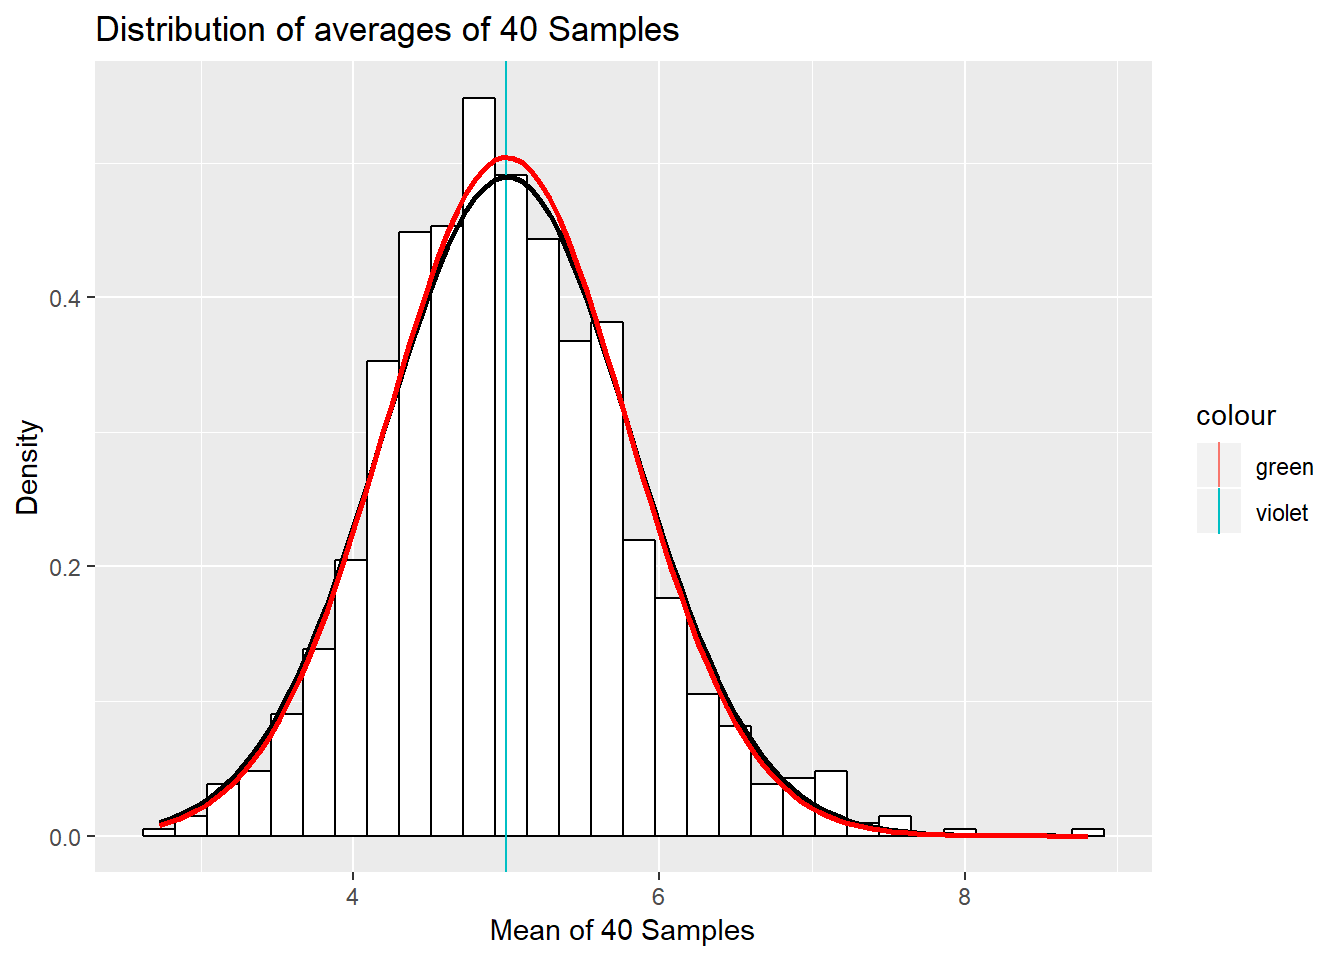
\includegraphics{Course6Assignment_files/figure-latex/unnamed-chunk-11-1.pdf}

The density of the actual data is shown by the light blue bars. The
theoretical mean and the sample mean are so close that they overlap. The
``red'' line shows the normal curve formed by the the theoretical mean
and standard deviation. The ``royal blue'' line shows the curve formed
by the sample mean and standard deviation.

As you can see from the graph, the distribution of averages of 40
exponential distributions is close to the normal distribution with the
expected theoretical values based on the given lambda.

\subsection{Confidence Interval
Comparison}\label{confidence-interval-comparison}

Check the confidence interval levels to see how they compare.

\subsubsection{Sample CI}\label{sample-ci}

Calculate the sample confidence interval; sampleCI = mean of x plus or
minus the .975th normal quantile times the standard error of the mean
standard deviation of x divided by the square root of n (the length of
the vector x).

\begin{Shaded}
\begin{Highlighting}[]
\NormalTok{sampleConfInterval <-}\StringTok{ }\KeywordTok{round}\NormalTok{ (}\KeywordTok{mean}\NormalTok{(simMeans) }\OperatorTok{+}\StringTok{ }\KeywordTok{c}\NormalTok{(}\OperatorTok{-}\DecValTok{1}\NormalTok{,}\DecValTok{1}\NormalTok{)}\OperatorTok{*}\FloatTok{1.96}\OperatorTok{*}\KeywordTok{sd}\NormalTok{(simMeans)}\OperatorTok{/}\KeywordTok{sqrt}\NormalTok{(n),}\DecValTok{3}\NormalTok{)}
\NormalTok{sampleConfInterval}
\end{Highlighting}
\end{Shaded}

\begin{verbatim}
## [1] 4.749 5.254
\end{verbatim}

\subsubsection{Theoretical CI}\label{theoretical-ci}

Calculate the theoretical confidence interval; theoCI = theoMean of x
plus or minus the .975th normal quantile times the standard error of the
mean standard deviation of x divided by the square root of n (the length
of the vector x).

\begin{Shaded}
\begin{Highlighting}[]
\NormalTok{theoConfInterval <-}\StringTok{ }\NormalTok{theoMean }\OperatorTok{+}\StringTok{ }\KeywordTok{c}\NormalTok{(}\OperatorTok{-}\DecValTok{1}\NormalTok{,}\DecValTok{1}\NormalTok{) }\OperatorTok{*}\StringTok{ }\FloatTok{1.96} \OperatorTok{*}\StringTok{ }\KeywordTok{sqrt}\NormalTok{(theoVar)}\OperatorTok{/}\KeywordTok{sqrt}\NormalTok{(n)}
\NormalTok{theoConfInterval}
\end{Highlighting}
\end{Shaded}

\begin{verbatim}
## [1] 4.755 5.245
\end{verbatim}

The sample confidence interval is \textbf{4.749 5.254} and the
theoretical confidence level is \textbf{4.755 5.245}. The confidence
levels also match closely. Again, proving the distribution is
approximately normal.

\subsection{Conclusion}\label{conclusion}

It is determined that the distribution does indeed demonstrate the
Central Limit Theorem; a bell curve. After graphing all the values above
and comparing the confidence intervals the distribution is approximately
normal.


\end{document}
